% quantgrav.tex - working draft.  Build:  make quantgrav   (writes build/quantgrav.pdf)
% Every number quoted in the text is a macro \qg... from build/quantgrav_numbers.tex, which models/paper_numbers.py writes from the models.
% Write negative numbers inside math mode ($...$) so that the minus sign is typeset as a minus.
\documentclass[11pt]{article}
\usepackage[T1]{fontenc}
\usepackage[utf8]{inputenc}
\usepackage{amsmath,amssymb,amsthm}
\usepackage{mathtools}
\usepackage[a4paper,margin=28mm]{geometry}
\usepackage{graphicx}
\usepackage{booktabs}
\usepackage{xcolor}
\usepackage{enumitem}
\usepackage{url}
\usepackage[hidelinks]{hyperref}
\usepackage{orcidlink}
\graphicspath{{figures/}}
\IfFileExists{build/quantgrav_numbers.tex}{\input{build/quantgrav_numbers.tex}}{\PackageError{quantgrav}{Run models/paper_numbers.py first (make quantgrav does)}{}}

% labels of evidence, used in every result
\newcommand{\exact}{\textbf{\textsc{Exact}}}
\newcommand{\numeric}{\textbf{\textsc{Numeric}}}
\newcommand{\hypo}{\textbf{\textsc{Hypothesis}}}
\newcommand{\negres}{\textbf{\textsc{Negative}}}
\newcommand{\snap}{\textsuperscript{$\dagger$}}      % number copied from a snapshot, not recomputed by paper_numbers.py
\newcommand{\todo}[1]{\textcolor{red}{[TODO: #1]}}
\setlength{\emergencystretch}{3em}
\theoremstyle{definition}
\newtheorem{result}{Result}


\title{Seam Automata, Phason Flips, and Dipolar Pair Qubits on the Spectre Monotile}

\author{Brent Hartshorn \orcidlink{0009-0004-2853-655X}, Tristan Romanov and James Lockwood}
\date{\today}

\begin{document}
\maketitle

\begin{abstract}
\noindent In the Spectre aperiodic monotile a tiling is a point of an internal space, and moving that point rearranges the tiles (a phason flip). We ask what a flip does and what Hamiltonian governs the two-valued degree of freedom, the position of the $14$th vertex, that the tile carries. Tiles that carry the bit come in bump-and-dent pairs. Their number obeys a linear recurrence of order five, the rule that places them on supertile boundaries is a finite table of $53$ types that closes at level $4$, and the patches of successive levels, and their pairs, are nested exactly ($6\subset82\subset804$ pairs). A flip is a cluster of tiles at uniform density that in three quarters of the tile-changing flips alters the contact graph, while the tetrad flux of the lift stays zero; the flip relation is symmetric, so it gives no arrow of time. The area ledger reduces each pair to one qubit with frustrated dipolar couplings, exactly solvable to $28$ pairs, whose entanglement peaks in a window that the Spectre--Hat flow crosses but does not grow with size. The relative entropy of a region follows its volume, not its boundary, no area observable of the model is proportional to it, and the local first law holds only for a hot reference state, whichever the sign of the temperature. Of the quantum-gravity diagnostics we apply (Pachner moves, tetrad flux, an area--relative-entropy relation, modular Hamiltonians), most give negative or limited answers, and we collect them in an appendix.
\end{abstract}

%------------------------------------------------------------------------------------------------------------------------------------
\section{Introduction}\label{sec:intro}
Discrete approaches to quantum gravity ask for a background whose elementary changes are local, reversible and rich enough to carry geometry: moves on a triangulation \cite{pachner1991}, rewrites of a graph. Aperiodic tilings have a ready-made family of such changes, which makes them a natural place to apply the diagnostics those approaches use; we do so as a test, not as a proposal of a theory of gravity. A tiling of the plane by the Spectre \cite{smith2023}, the strictly chiral aperiodic monotile, is a model set: a tile is present iff the internal image of its lattice vector lies in a fractal window \cite{bgms}. Moving the internal phase by a small step (a \emph{phason step} \cite{socolar1986}) removes tiles near the window boundary and adds others elsewhere; the ordered pair of phases is a \emph{flip}. The Spectre also carries a natural two-valued degree of freedom, the position of its $14$th vertex, which becomes a qubit once the tiling's area ledger is imposed.

The paper has two parts: exact combinatorics and flip dynamics of the tiling, and quantum information and statistical mechanics of the qubits it carries. Equation~\eqref{eq:overview} is the whole paper in one line.

The whole paper is one pipeline, read from the top: a substrate fixes what a flip is, the tile's bit gives a Hamiltonian, the Hamiltonian's states are tested against relative entropy and a Hopf structure, and what is left over is stated as hypotheses.

{\scriptsize
\begin{equation}\label{eq:overview}
\mathcal{P}_{\text{pair-qubit}}
\;=\; \left\{ \begin{aligned}
&\text{I. Substrate.}\quad (b,u{+}w)\ \text{present at phase } z \iff B_b\,z+d_{b,w}\in Z_0(S_b),\qquad \lambda^2=4+\sqrt{15} \\
&\qquad \text{(Results~\ref{res:window-pieces}, \ref{res:index36})} \\
&\Downarrow\quad \text{(phason step } z\mapsto z'=z+\delta e \text{)} \\
&\text{II. Flip.}\quad \mathcal{F}(z,z')=\mathcal{T}(z)\triangle\mathcal{T}(z')=\mathcal{F}(z',z),\qquad \mathbb{E}\,|\mathcal{F}\cap D_\rho|\propto\rho^{2.25} \\
&\qquad G(z)\not\cong G(z')\ \text{in } 75\%\ \text{of tile-changing flips},\qquad F^{\hat\alpha}=0\ \text{on every flip of the lift} \\
&\qquad \text{(no arrow; Results~\ref{res:flip-symmetry}, \ref{res:flip-density}, \ref{res:flip-contact}, \ref{res:lift-flux})} \\
&\Downarrow\quad \text{(the bit: } P_8 \text{ at } \pm h \text{ moves area } \pm a h \text{ inside a pair; ledger } Q=\sigma^z_i+\sigma^z_j=0 \text{)} \\
&\text{III. Pairs.}\quad P_k=0,0,6,82,804,\dots\ \text{(order-5 recurrence)},\qquad \text{placement rule: 53 types, closed at level 4} \\
&\qquad \text{(Results~\ref{res:found-pairs-proof}, \ref{res:ham-rg-closed})} \\
&\Downarrow\quad \text{(one qubit } \tau_A \text{ per pair, along the Spectre--Hat flow } \tau\in[0,1]\text{)} \\
&\text{IV. Hamiltonian.}\quad H(\tau)=-J(\tau)\sum_{A}\tau^x_A-\kappa(\tau)\sum_{A<B}W_{AB}\bigl(b(\tau)\bigr)\,\tau^z_A\tau^z_B \\
&\qquad W_{AB}=\tfrac1{r_{AA'}}-\tfrac1{r_{AB'}}-\tfrac1{r_{BA'}}+\tfrac1{r_{BB'}}\ \propto r^{-3}\ \text{(frustrated dipoles)};\quad \text{Eq.~\ref{eq:hbit}; Results~\ref{res:ham-pair}, \ref{res:flow-patch}, \ref{res:ham-flow}} \\
&\qquad h(\tau)=\tan\bigl(60^\circ(1-\tau)\bigr),\quad J=e^{-h^2/2},\quad \kappa=\kappa_{\mathrm{norm}}h^2,\quad b(\tau)=1+(\sqrt3-1)\tau \\
&\Downarrow\quad \text{(ground state } \psi(\tau) \text{ and its reduced states } \rho_A \text{)} \\
&\text{V. Entanglement and relative entropy.}\quad C_{pq}\ \text{peaks at } \tau_{\mathrm{eff}}\in[0.4,1.2],\ \text{no growth with size} \\
&\qquad S_{\mathrm{rel}}(\rho_A\|\sigma_A)=\mathrm{Tr}\,\rho_A(\ln\rho_A-\ln\sigma_A)\ \propto\ \text{volume and } \delta^2,\ \text{not area (ledger neutral, bump area linear)} \\
&\qquad K_A=-\ln\rho_A\approx\beta_{\mathrm{eff}}H_A\ \text{only for } |\beta|\lesssim 0.5 \\
&\qquad \text{(Results~\ref{res:ent-flow}, \ref{res:rel-volume}, \ref{res:rel-area}, \ref{res:rel-thermal}, \ref{res:rel-profile})} \\
&\Downarrow\quad \text{(a pair of pair qubits, and the nested levels)} \\
&\text{VI. Hopf structure.}\quad (q_1,q_2)\in S^7\ \mapsto\ (2q_1\bar q_2,\ |q_1|^2-|q_2|^2)\in S^4:\quad |\vec r_1|^2+C^2=1 \\
&\qquad D=(1-|\vec r_p|^2)-C_{pq}^2\ge0\ \text{(zero for a pure pair)} \\
&\qquad \text{levels nest exactly } (6\subset82\subset804);\ I(\text{shell}_i{:}\text{shell}_j)\ \text{no larger than for a random grouping} \\
&\qquad \text{(Results~\ref{res:nesting}, \ref{res:hopf-s4}, \ref{res:hopf-leak}, \ref{res:hopf-tiers})} \\
&\Downarrow\quad \text{(hypotheses, not tested)} \\
&\text{VII. Candidates.}\quad \kappa\ \text{derived from the geometry} \\
&\qquad \text{a hierarchy effect in the entanglement of the nested levels at } 82 \text{ and } 804 \text{ pairs} \\
&\qquad \delta A\overset{?}{=}4G\,S_{\mathrm{rel}}\ \text{\cite{doraumuch}};\quad (dV,dE,dF)\overset{?}{\in}\text{Pachner moves}
\end{aligned} \right.
\end{equation}
}

Rows I to VI are exact or measured and row VII is not. Rows I to III are exact or enumerated; row IV is the Hamiltonian of the bits, with couplings $W_{AB}$ computed from the exact tile geometry at every $b$ and scales $J$, $\kappa$, $h$ from the Spectre--Hat flow; rows V and VI are what its ground state says about entanglement, relative entropy and the Hopf structure of two qubits, mostly negatively. Nothing in Eq.~\eqref{eq:overview} is a derivation of gravity.

\emph{Related work.} Connectivity changes of a gravitational field in tetrad form are studied by Comisso and Asenjo \cite{comisso2026}; we test the nearest discrete statement (Appendix~\ref{app:neg}). Arrows of time from structure are studied in the Janus-point programme \cite{barbourlobo2026}. Frustrated constraints and quantum constraint satisfaction are reviewed in \cite{gharibian2015}; a local Hamiltonian cannot be credited with more than Tsirelson's bound \cite{cirelson1980}.

\emph{Conventions.} Every result carries one label: \exact\ (an identity, a proof or a finite enumeration checked by a test that can fail), \numeric\ (a computed number on a finite patch), \negres\ (a natural expectation that the computation refutes) or \hypo\ (not shown). Numbers marked $\dagger$ are copied from a log or snapshot; all others are written into the text from the code, which checks $\qgTNumbersChecked$ of them on every build. The code and the command that rebuilds everything are in Appendix~\ref{app:repro}.

%------------------------------------------------------------------------------------------------------------------------------------
\section{The substrate and the bit}\label{sec:model}
The Spectre has $14$ edges of unit length at multiples of $30^\circ$ \cite{smith2023}; the Hat \cite{smith2024hat} belongs to the same two-parameter family. In the lift of Ch\'eritat and Ma \cite{cheritat2023} a vertex is an integer vector $(p,q,r,s)$ with plane position $u+\zeta v$, $u=p+q\varpi$, $v=r+s\varpi$, $\varpi=e^{i\pi/3}$, $\zeta=e^{i\pi/6}$; all exact computations use these integer vectors. The vertices form a model set: a tile $(b,u{+}w)$ of class $b$ is present at internal phase $z$ iff $B_bz+d_{b,w}\in Z_0(S_b)$, where $Z_0$ is a window with fractal boundary.
\begin{result}[\exact, source]\label{res:window-pieces}
The window of a tile of shape $O$ (the tile) or $G$ (the two-tile ``Gamma'' shape) in the frame of parity $p\in\{0,1\}$ is an attractor of a graph-directed system of similarities of ratio $1/\lambda$, $\lambda^2=4+\sqrt{15}$ ($\lambda=\qgKLam$). The pieces $Z_0(O)$, $Z_1(O)$, $Z_0(G)$, $Z_1(G)$ have $\qgKPieces$ children, and the seams between the children have box dimension $\log(5+2\sqrt6)/\log(4+\sqrt{15})=\qgKSeam$ (a lower bound for the boundary dimension of the window). We rasterise these maps and do not re-prove them.
\end{result}
\begin{result}[\exact\snap]\label{res:index36}
The tile vectors of every window class of the level-$3$ patch lie in a coset of one sublattice of $\mathbb{Z}^4$ of index $\qgKIndex$ (Smith normal form $1,1,6,6$; $\qgKTilevec$ tile vectors, $\qgKClasses$ classes). A placement $(b,w)$ is possible only if $w\equiv v_b-u_a$ modulo that sublattice.
\end{result}
A \emph{phason step} replaces $z$ by $z'=z+\delta e$, $|e|=1$, and a \emph{flip} is the ordered pair $(z,z')$ when the set of present tiles $\mathcal{T}$ changes, with content $\mathcal{F}(z,z')=\mathcal{T}(z)\triangle\mathcal{T}(z')=\mathcal{F}(z',z)$.

Of the $14$ vertices the eighth, $P_8$, is flat in the straight outline. In the model it carries a bit $s=\pm1$: with $s=+1$ it stands out of the chord $P_7P_9$ by $h$ (a convex tile), with $s=-1$ it stands in by $h$ (a reflex tile). On a tiling a tile can open only together with a partner, two tiles whose eighth vertices meet alone, a \emph{bump-and-dent pair}. The \emph{area ledger} $Q=\sigma^z_i+\sigma^z_j=0$ holds for the pair, which turns the two bits into one qubit (Section~\ref{sec:ham}).

%------------------------------------------------------------------------------------------------------------------------------------
\section{Exact combinatorics of the pairs}\label{sec:pairs}
Let $T_k$ be the number of tiles of the level-$k$ patch ($1,9,71,559,4401,34649$ at levels $0$ to $5$, $T_k=8T_{k-1}-T_{k-2}$) and $P_k$ its number of bump-and-dent pairs ($\qgWPairsTwo$, $\qgWPairsThree$, $\qgWPairsFour$ at levels $2,3,4$).
\begin{result}[\exact]\label{res:found-pairs}
$T_k=A\mu^k+B\mu^{-k}$ with $\mu=4+\sqrt{15}$, and the counts $P_k=0,0,6,82,804,7012,58106,\qgWPairSeven$ for $k=0,\dots,7$ satisfy a recurrence with characteristic polynomial $(x-1)(x^2-8x+1)(x^2-4x-1)$: the roots are those of the tile counts ($\mu^{\pm1}$) and of the perimeter law of the supertiles ($\nu=2+\sqrt5=\varphi^3$, $2-\sqrt5$, and $1$). The recurrence holds for every $k$ (Result~\ref{res:found-pairs-proof}). From it
\[
P_k=\frac{\mu^k-\mu^{-k}}{\sqrt{15}}-\Bigl(\tfrac14+\tfrac{3\sqrt5}{20}\Bigr)\nu^k-\Bigl(\tfrac14-\tfrac{3\sqrt5}{20}\Bigr)(2-\sqrt5)^k+\tfrac12,
\]
so $P_k/T_k\to2/(5+\sqrt{15})=(5-\sqrt{15})/5=\rho_0=\qgRhoZero$, the density of valence-$4$ vertices, with a correction of order $(\nu/\mu)^k=\qgWBoundaryRatio^k$. At level $3$, $\qgWPairPctThree\%$ of the tiles are in a pair.
\end{result}
\begin{result}[\exact]\label{res:found-pairs-proof}
The recurrence of Result~\ref{res:found-pairs} holds for every $k$. Call $O$ any of the eight species other than $\Gamma$, and $G$ the species $\Gamma$. By induction on $k$ the eight species $O$ have the same tile set, outline and flat-pair count $P_k(O)$, because their substitution rules differ only in the species of the children; $\Gamma$ omits the child in slot $2$ and has $P_k(G)$. Write the seam of two adjacent children as a relative transform in $\mathbb{Z}[\omega]^4$, $\omega=e^{i\pi/3}$. The reflection $R=-\overline{(\cdot)}$ cancels in every transform between children of the same level, and the reachable seams close on $15$ states ($13$ occur in $O$, $11$ in $G$) with an integer transition matrix $M\in\mathbb{Z}^{15\times15}$. No triple junction creates a flat pair, so $P_{k+1}(O)=7P_k(O)+P_k(G)+J_{k+1}(O)$ and $P_{k+1}(G)=6P_k(O)+P_k(G)+J_{k+1}(G)$, where $J_k$ counts the pairs across seams and is linear in $M^k\mathbf b_1$. The Krylov space of $\mathbf b_1$ under $M$ has dimension $4$ (eigenvalues $2\pm\sqrt5$, $+1$, $-1$), and the $(-1)^k$ mode vanishes in the read-out of both $O$ and $G$, so $J_k$ has minimal polynomial $(x-1)(x^2-4x-1)$ for $k\ge2$, and $P_k$ the polynomial above for all $k\ge0$ ($O$) and $k\ge1$ ($G$).
\end{result}
The computation uses exact integer and rational arithmetic (closure of the automaton, the Krylov dimension and the counts to level $7$; code in Appendix~\ref{app:repro}); the step to all $k$ is the closure of the automaton, which no second independent program has confirmed.
\begin{result}[\exact\snap]\label{res:nesting}
The patches of successive levels are nested exactly. The level-$k$ patch of a species is the union, over the eight slots of the substitution, of the level-$(k{-}1)$ patches of the child species of that slot, each moved by the slot transform. For the single-tile species the child of slot $1$ is again the single-tile species, so the level-$(k{-}1)$ patch is, as a set of exact leaf tiles, the image of itself under that slot transform inside the level-$k$ patch ($9\subset71\subset559\subset4401$ tiles for $k=2,3,4$, checked by comparing the exact integer transforms of every tile); the Mystic species nests the same way through its slot $7$ ($8\subset62\subset488\subset3842$). Every flat pair of level $k$ is a flat pair of level $k+1$ ($6\subset82\subset804$ pairs). So a pair qubit of a small patch is a pair qubit of every larger one, and the levels are nested regions of one tiling, not separate systems.
\end{result}
\subsection{The local pair rule}\label{sec:rule}
No flat pair lies inside a block (a level-$L$ supertile of one tile of the level-$(L{-}1)$ patch), every pair of level $L-1$ reappears as one pair of level $L$, and the others lie on boundaries between adjacent blocks.
\begin{result}[\exact\snap\ for levels $2$ to $6$]\label{res:ham-rg-closed}
Give each tile its leaf label, the species $c$ of the tile it was created as (a tile of species $c$ is inflated into the supertile of species $c$), and its kind (single, or one of the two halves of a Mystic pair). The type of the seam between two adjacent blocks is the two labels with the shared edge pairs, taken up to exchange of the blocks; its count is the number of flat pairs on the seam. At levels $2$ to $6$ ($6$, $82$, $804$, $7012$, $58106$ pairs) no pair lies inside a block or joins blocks that are not adjacent, a seam carries at most one pair, and the count is a function of the type. The numbers of types are $14$, $46$, $53$, $53$, $53$ ($6$, $28$, $35$, $35$, $35$ of them with a pair), and the sets at levels $4$, $5$, $6$ are equal: no new type appears after level $4$. Keyed instead by the outermost species of the tile (a position in the whole hierarchy, not a property of the block) the table does not close ($\qgZTypesFour$ types at level $4$, $\qgZTypesNew$ of them new).
\end{result}
\hypo: no new type appears at any level (a proof would need the seam automaton to determine the type). The table was rebuilt from a previously reported one, which has $66$ types when blocks are ordered by index and $53$ up to exchange.

\subsection{Orientation parity}
\begin{result}[\exact\snap]\label{res:flip-parity}
The minority parity counts $1,8,63,496,3905$ at levels $1$ to $5$; the count at one level is the majority count at the previous one, and the minority frequency tends to $(5-\sqrt{15})/10=0.11270$ with ratio majority to minority $4+\sqrt{15}=\lambda^2$. Hence the window of a Mystic pair has $1/(3+\sqrt{15})=0.14550$ of the area of a single tile's window; \numeric: measured $0.1578$, $0.1515$, $0.1479$, $0.1460$ at tolerances $0.012$, $0.006$, $0.003$, $0.0015$. The orientation frequencies are window areas.
\end{result}

%------------------------------------------------------------------------------------------------------------------------------------
\section{Phason flips}\label{sec:flips}
We follow the tile of class $0$ at the origin of a level-$3$ patch (placement engine and tolerances in Appendix~\ref{app:neg}). All numbers marked $\dagger$ in this section are for one class, one footprint and one patch, so none is a statement about all tilings.
\begin{result}[\numeric\snap]\label{res:flip-clusters}
One phase changes about $10$ tiles in a region of radius $14$ about the origin tile (mean $9.9$ removed, median $11$, at most $37$), uniformly in distance: the frequency of change per placement is $0.0021$, $0.0020$, $0.0022$, $0.0022$, $0.0023$ in the shells $0$--$3$, $3$--$6$, $6$--$9$, $9$--$12$, $12$--$14$. Linking removed and added tiles that overlap gives $818$ clusters; the first twelve inspected have $8$ to $17$ tiles on each side and areas $80$ to $172$ (Figure~\ref{fig:flip-gallery}). The tile count differs by one where a Mystic pair is exchanged for two single tiles. No cluster satisfies the closure test, because the region in which the placement list is complete (radius $8.5$) is smaller than the clusters.
\end{result}
\begin{result}[\numeric\snap]\label{res:flip-density}
The mean number of changed tiles inside a disc of radius $\rho$ about the tile grows as $\rho^{2.25}$ ($\rho=1.5$ to $7$, $2831$ usable phases), and the number of changed tiles per tile present is constant, $0.056$ at every $\rho$ (a lower bound, since phases inside the ambiguity band are dropped).
\end{result}
\begin{figure}[t]\centering
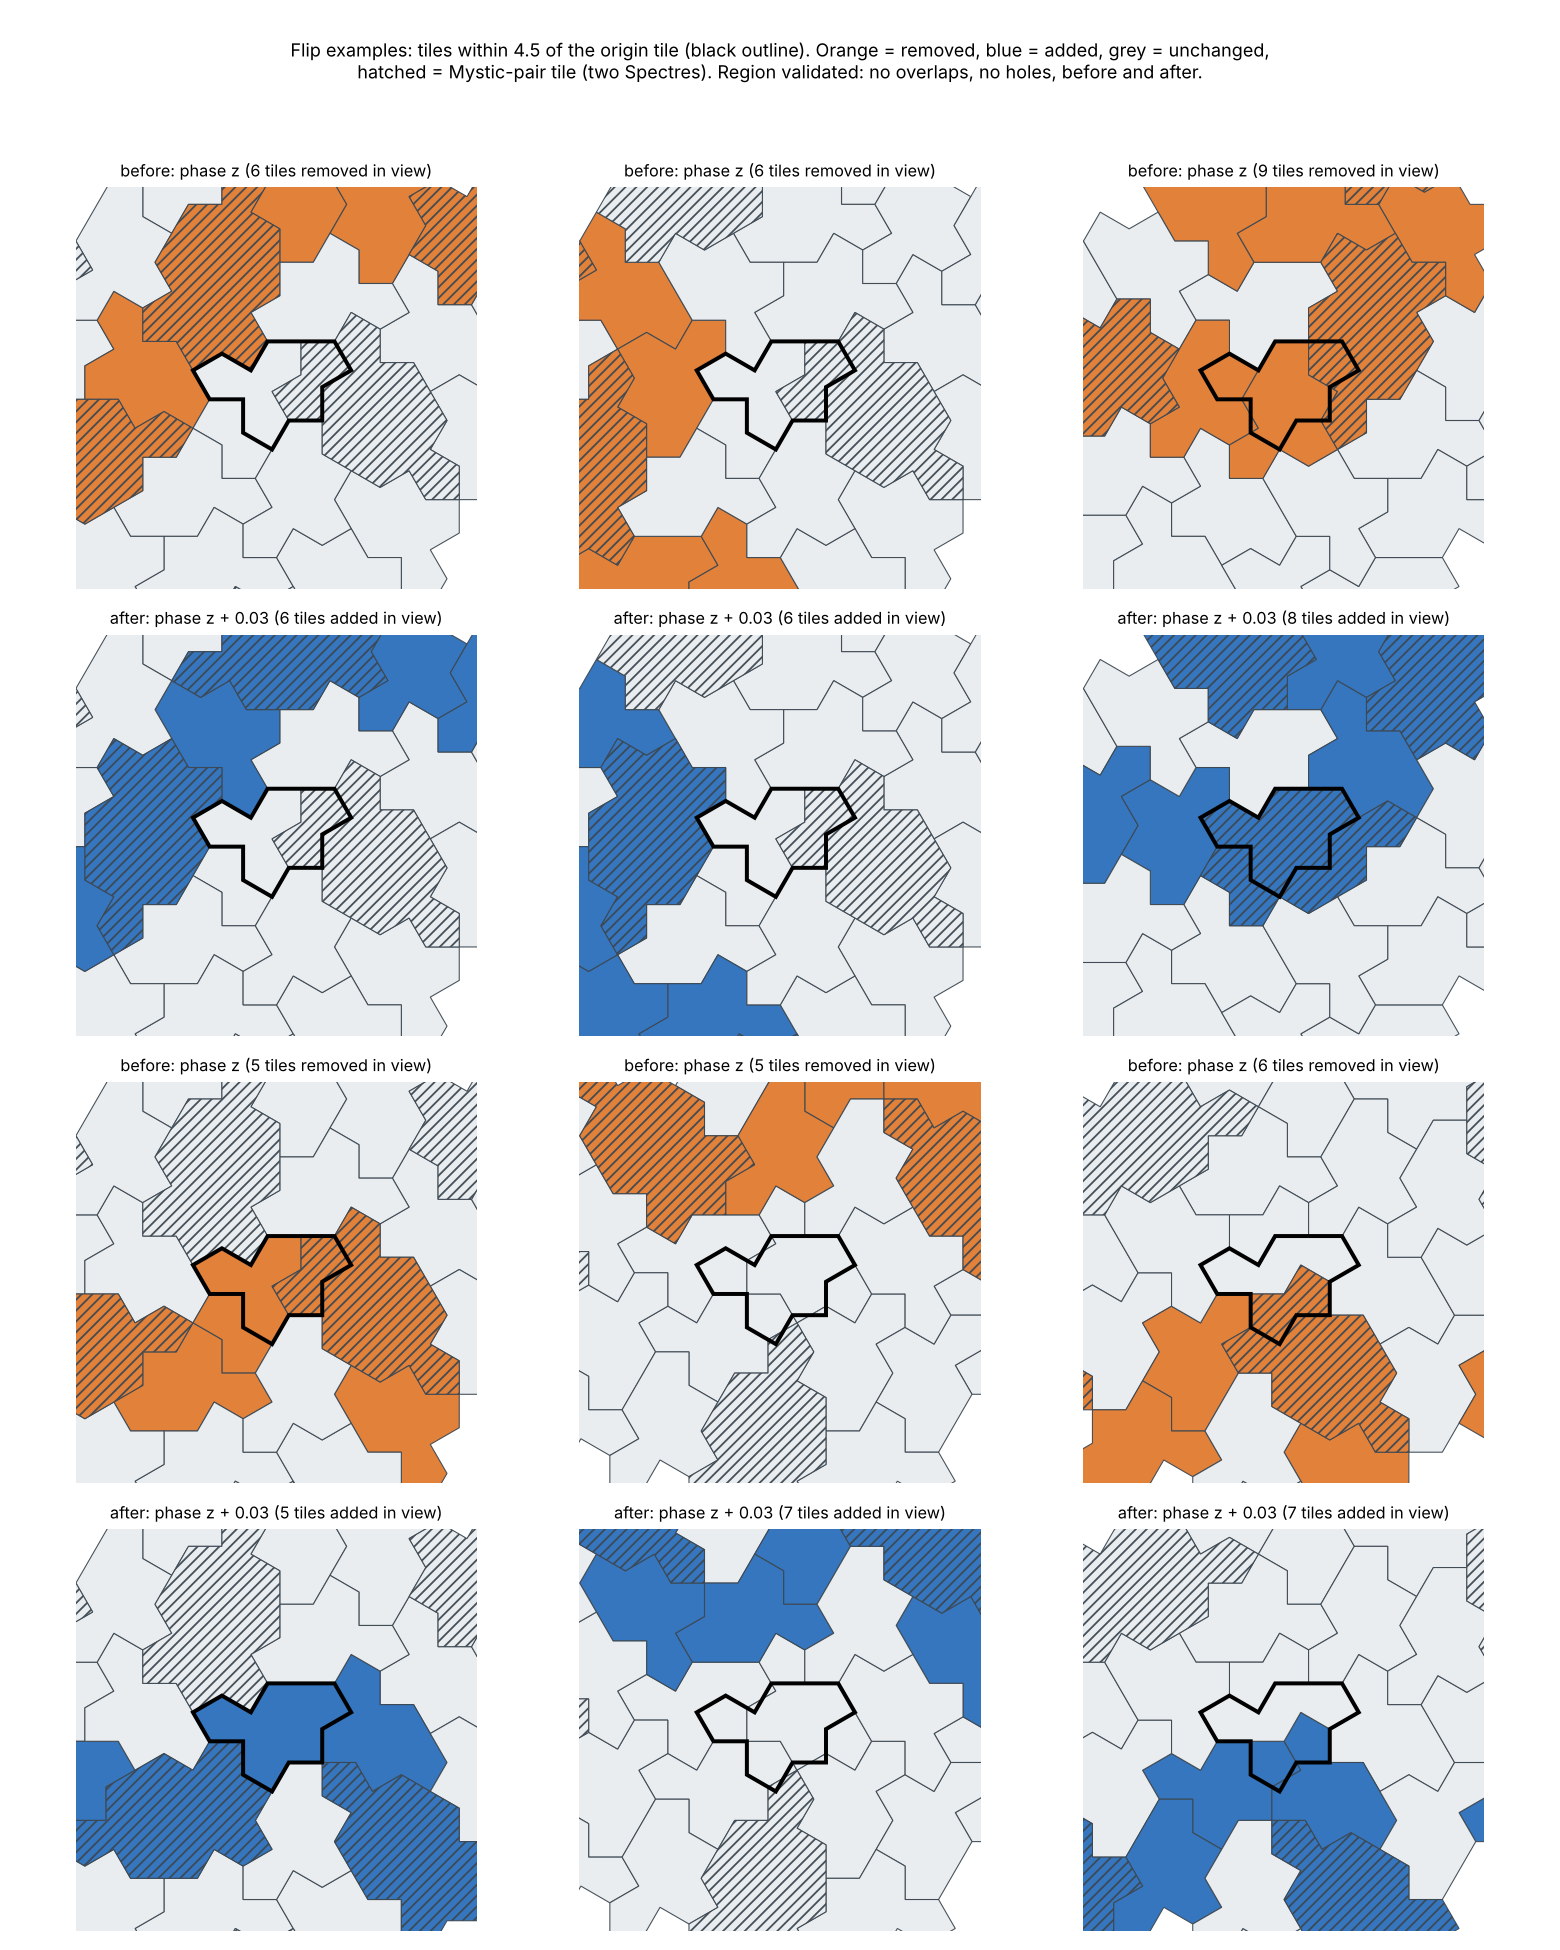
\includegraphics[width=\linewidth]{research/toymodel_v8/figures/fig_flip_gallery.png}
\caption{Four flips picked at random among $416$ validated events that touch the footprint (class $0$, level $3$, $\delta=0.03$). Black: the tile at the origin; orange: present before and not after; blue: present after and not before; hatched: Mystic-pair tiles. In each panel the region within $4.5$ of the origin tile has no overlap and no hole before and after.}\label{fig:flip-gallery}
\end{figure}

\subsection{The contact graph changes; the field sheets do not}\label{sec:flips-contact}
The footprint is the origin tile enlarged by a margin of $1$ ($767$ placements); the graph has the tiles meeting the footprint as vertices and contact along an edge as links.
\begin{result}[\numeric\snap]\label{res:flip-contact}
Of $6000$ phases ($5245$ unambiguous) $539$ change the present set, and $468$ of these have a valid tiling before and after. In $224$ ($48\%$) the set of tiles meeting the footprint changes, and in $169$ of those ($75\%$) the contact graph is not isomorphic before and after; in $55$ it is isomorphic as an unlabelled graph and differs in the classes. The reversed step gives identical counts.
\end{result}
\begin{result}[\exact; \hypo\ for the identification]\label{res:lift-flux}
Identify the four components of a tetrad index with the four coordinates of the lift lattice $\mathbb{Z}^4$ (this identification is ours). The edge vectors of any tiling that is a lift are differences of lattice points, so the one-forms $A^{\hat\alpha}$ are exact and the field strength $F^{\hat\alpha}=dA^{\hat\alpha}$ is zero on every closed loop of the tiling graph, for every phase. A phason flip, which changes which tiles touch, leaves every flux equal to zero: every direction is annihilated by $F$, the field sheets are trivial and there is nothing to reconnect.
\end{result}
The two notions of connectivity therefore disagree on the same flips. This does not make a flip a reconnection in the sense of Comisso and Asenjo \cite{comisso2026}.

\subsection{No arrow of time; exact refilling}
\begin{result}[\exact; \negres]\label{res:flip-symmetry}
The present set at a phase is a function of the phase, and ``the region is tiled without overlap or hole'' and ``the two contact graphs are isomorphic'' are symmetric in the two phases. So $(z,z')$ is a valid flip iff $(z',z)$ is, and every count of flips by type is identical in the two orientations. \numeric\snap: the reversed run of Result~\ref{res:flip-contact} reproduces all counts.
\end{result}
An arrow would need an initial condition, a rate violating detailed balance, or the direction of the inflation (which changes the relative size of a step by $\lambda$ per level); none was found, and the last was not tested.
The point cloud cannot say whether a cluster of changed tiles is a tiling, so we ask exactly on the level-$4$ patch: erase $k$ tiles and list every filling of the hole by Spectres, edge to edge and without overlap, by a search over open vertices with an exact test over $\mathbb{Q}(\sqrt3)$.
\begin{result}[\exact\snap\ for the holes tried]\label{res:flip-cavity}
For the $k$ tiles nearest to a central tile, $k=1$ (all twelve orientations), $10$, $20$, $40$, $80$, $150$ and $300$ (radius $27.96$), the only filling is the original. Every step is forced: the search visits $k+1$ nodes for $k\le40$ and $88$, $170$, $371$ nodes for $k=80$, $150$, $300$ ($8$ minutes at $k=300$). So no flip of the tiles of such a hole exists that leaves the rest of the patch fixed.
\end{result}
This does not say that the clusters of Result~\ref{res:flip-clusters} are absent: they may reach outside the hole. An independent SAT computation (CaDiCaL, certificates checked with \texttt{drat-trim}) reports the same uniqueness to $300$ tiles and, in addition, a $2$-tile swap at $k=4$ when reflected tiles are allowed; we do not reproduce that swap, and the holes of the reported swap were not available to us. In two dimensions two triangulations of one surface are related by a finite sequence of bistellar moves \cite{pachner1991}, so ``a flip is a composite of local moves'' is nearly automatic; what would carry information is the length of the word, and no closed cluster was reached. Whether the absence of ambiguous erasure (Appendix~\ref{app:neg}) is a code in the sense of a Landauer-type cost \cite{landauer1961} would need a record of the erased tile, which was not modelled.

%------------------------------------------------------------------------------------------------------------------------------------
\section{A Hamiltonian for the bits}\label{sec:ham}
Put a qubit on each tile, $\sigma^z=+1$ convex and $-1$ reflex. With the area ledger as a penalty,
\begin{equation}\label{eq:hbit}
H=-J\sum_{\mathrm{pairs}}\sigma^x_i\sigma^x_j+g\sum_{\mathrm{pairs}}(\sigma^z_i+\sigma^z_j)^2-\sum_{A<B}K_{AB}\,\sigma^z_{A_1}\sigma^z_{B_1}-\varepsilon\sum_i\sigma^z_i .
\end{equation}
\begin{result}[\exact]\label{res:ham-pair}
$\sigma^x_i\sigma^x_j$ flips both tiles of a pair, so it commutes with $Q^2$: the sector $Q=0$ is invariant for every $g$, and in it each pair is one qubit $\tau$ with $H_{\mathrm{eff}}=-J\sum\tau^x-\sum K_{AB}\tau^z_A\tau^z_B$; no limit $g\to\infty$ is needed. The uniform field vanishes on the sector, so the area term cannot bias a pair. One pair cannot violate CHSH: the only one-tile observables that commute with the ledger are functions of $\sigma^z$. For two pairs the ground state has concurrence $C=K/\sqrt{4J^2+K^2}$ \cite{wootters1998} and largest CHSH value $2\sqrt{1+C^2}$ \cite{horodecki1995}.
\end{result}
\subsection{Frustrated dipoles on patch clusters}\label{sec:ham-patch}
On a patch the pairs are disjoint and the same along the flow, so each carries a pair qubit. The coupling is not chosen: with the bit read as a charge $\pm h$ at the centroid of its tile, a pair is a dipole and $K_{AB}$ is the Coulomb energy of two dipoles.
\begin{result}[\exact; \negres\ for the two-pair picture]\label{res:ham-patch}
The charges give an exact Ising coupling with both signs ($\qgYAntiFour$ of the couplings antiferromagnetic at level $4$), falling as $r^{-3}$ (fitted slope $\qgYSlope$). The patch is frustrated: the classical ground state leaves $\qgYFrusTwo$ of the bond weight unsatisfied on the six pairs of level $2$, and $\qgYFrusLo$ to $\qgYFrusHi$ on the central $6$ to $14$ pairs of level $3$. As the tunnelling goes to zero, the ground state of every such cluster is the cat $(|s\rangle+|{-s}\rangle)/\sqrt2$ of its classical ground state $s$, whose two-pair reductions have concurrence below $10^{-10}$. For two pairs that cat is a Bell state, which is why the two-pair model is most entangled at the Spectre end.
\end{result}
\begin{result}[\exact\snap; \numeric\snap]\label{res:ham-dipole-large}
Result~\ref{res:ham-patch} continues beyond $14$ pairs. The exact ground state of the $N$ central pairs of level $3$ (all $2^{N-1}$ states, split in two blocks, Python with \texttt{numpy}) is unique up to the global flip for every even $N$ from $6$ to $28$, with unsatisfied weight $f=0.1649$ at $N=14$ and $0.1695$, $0.1723$, $0.1937$, $0.2046$, $0.2062$, $0.2111$, $0.2091$ at $N=16,\dots,28$; $f$ is not monotone in $N$. Annealing with descent agrees with the exact value at $N=14$ and $20$. Beyond that it gives upper bounds only, $f\le0.2293$ for the whole level-$3$ patch ($N=82$) and $f\le0.294$ for level $4$ ($N=804$), and the best energy is reached by one restart of $32$ to $128$, so these are not converged. \hypo: that $f$ tends to a bulk value near $0.29$.
\end{result}

\subsection{Along the Spectre--Hat flow}\label{sec:flow}
A parameter $\tau\in[0,1]$ moves the tile from the Spectre to the Hat: $b(\tau)=a(1+(\sqrt3-1)\tau)$, and the bit sits at $\pm h(\tau)$ from the chord.
\begin{result}[\exact]\label{res:flow-area}
The area of the tile splits as $A_\pm=A_0(b)\pm ah$ with $A_0=2\sqrt3a^2+3ab+\sqrt3b^2$ independent of $k$ and $\omega$: the two bit values differ by $a$ times the jump $d=2h$ and by nothing else, and give the same tile iff $\omega=0$ (proof in Appendix~\ref{app:proofs}). At $\omega_0=120^\circ$, $a=1$: $d(0)=\qgWJumpZero$, $d(1/2)=\qgWJumpHalf$.
\end{result}
\begin{result}[\exact\snap]\label{res:flow-patch}
Along the flow the tiling does not change: every vertex keeps its integer vector $(p,q,r,s)$ and moves to $x_b=(p+q\varpi)+b\,\zeta\,(r+s\varpi)$, which is the Tile$(1,b)$ geometry. In the patches of levels $2$ to $4$ the tiles of the minority orientation parity (Result~\ref{res:flip-parity}) are exactly the tiles with the edge lengths of Tile$(b,1)$ ($8$, $63$, $496$ of $71$, $559$, $4401$; $496/4401=0.1127017$ against $(5-\sqrt{15})/10=0.1127017$) and every other tile is Tile$(1,b)$, with areas $A(b,1)$ and $A(1,b)$ ($A(1,\sqrt3)=8\sqrt3$, $A(\sqrt3,1)=10\sqrt3$). Every flat pair consists of two Tile$(1,b)$ tiles, so the area ledger of a pair is $2A(1,b)$ at every $b$ and a bit moves area between its two tiles and nowhere else. The dipole couplings of the $14$ central pairs of level $3$ computed this way agree with an independent patch code to $10^{-14}$ at $b=1.2,1.5,\sqrt3$. The closed forms for the areas and the Mystic fraction are exact statements in $\mathbb{Q}(\sqrt3)$ and $\mathbb{Q}(\sqrt{15})$, checked here by the numerical agreement above.
\end{result}
\begin{result}[\numeric\snap]\label{res:ent-flow}
Write $\tau_{\mathrm{eff}}=J/(\kappa w)$, with $w$ the rms nearest-neighbour coupling. In an exact scan of $6$ to $16$ central pairs (level $3$, level $4$ for $16$) the largest pairwise concurrence peaks at $\tau_{\mathrm{eff}}$ of $0.4$ to $1.2$ for every size, below which the ground state is the cat of Result~\ref{res:ham-patch}; but it does not grow with size ($0.38$, $0.52$, $0.65$, $0.51$, $0.44$, $0.35$ at $6$, $8$, $10$, $12$, $14$, $16$ pairs) and the CHSH value above $2$ (up to $2.33$ at $10$ pairs) is gone at $16$. We read this as a finite-size effect with monogamy as the cluster grows, not as a phase or a persistent Bell-violating network. With the flow definitions ($h(\tau)=\tan(60^\circ(1-\tau))$, $J=e^{-h^2/2}$, $\kappa=\kappa_{\mathrm{norm}}h^2$ with the strongest coupling of level $2$ at the Spectre end equal to $1$) and the couplings recomputed at $b(\tau)$ (Result~\ref{res:flow-patch}), the flow starts at $\tau_{\mathrm{eff}}=0.244$ and crosses the window. For the ten central pairs of level $3$ the largest concurrence is $0.407$ at $\tau=0$ and $0.565$, $0.647$, $0.619$, $0.509$, $0.354$, $0.202$ at $\tau=0.02$, $0.05$, $0.08$, $0.13$, $0.2$, $0.3$, the best CHSH value $2.10$, $2.33$ (at $0.05$) and $2.03$ (at $0.3$), and the gap of the even sector $0.092$ to $1.958$; Recomputing the couplings from the exact vertices reproduces these numbers to the six printed digits. Rescaling the $b=1$ couplings by $(h/h_0)^2$ instead of recomputing them gives a coupling matrix off by $0.7\%$ at $\tau=0.05$ and $4\%$ at $0.3$, and a largest concurrence off by at most $0.014$. A parameter set outside the window, $J=1$, $\kappa=0.09$, $h=0.3$, sits at $\tau_{\mathrm{eff}}=190$ to $260$: a product state.
\end{result}

%------------------------------------------------------------------------------------------------------------------------------------
\section{Relative entropy and the area ledger}\label{sec:rel}
Dorau and Much \cite{doraumuch} derive the semiclassical Einstein equations from the Araki--Uhlmann relative entropy $S(\rho\|\sigma)=\mathrm{Tr}\,\rho(\ln\rho-\ln\sigma)$ \cite{umegaki1962,araki1976}; the same programme on the Nariai horizon (source in Appendix~\ref{app:repro}) gives a relation in which $S_{\mathrm{rel}}=2\pi\,\delta Q$ is the boost energy of the excitation weighted by the modular flow and $\delta A=4G\,S_{\mathrm{rel}}$. Three ingredients are testable on the pair qubits: (i) whether the relative entropy of a region follows its boundary; (ii) whether an area observable of the model is proportional to it; (iii) whether the modular Hamiltonian $K_A=-\ln\rho_A$ of a region is a local energy, as it is for a wedge by the Bisognano--Wichmann theorem \cite{bisognano1975}. The reference is the ground state (or a Gibbs state) of the flow Hamiltonian at flow time $0.05$ for the central pairs of level $3$; entropies are in nats; numbers are copied from logs ($\dagger$).
\begin{result}[\numeric\snap; \negres\ for an area law]\label{res:rel-volume}
For $8$ to $14$ pairs, the relative entropy $S(\rho_A(\tau+\delta)\|\rho_A(\tau))$ of compact and random regions $A$ for a flow step $\delta=0.004$ follows the number of pairs, not the boundary: the volume-only fit has rms $0.0003$ to $0.0011$ nats against $0.0007$ to $0.0015$ for the Delaunay boundary alone, and with both regressors the boundary coefficient is zero or slightly negative ($-0.0001$ to $-0.0003$ against $+0.0006$ to $+0.0013$ for the volume). This is the response of an extensive Hamiltonian to a uniform change of its couplings, so it says nothing about the area law of the entropy itself. It scales as $\delta^2$ (the ratio is $3.5$ to $4.5$ when $\delta$ is halved), while the change of the tile area of the region, $2m\,[A(1,b(\tau+\delta))-A(1,b(\tau))]$, is first order in $\delta$; for a region of three pairs $S_{\mathrm{rel}}/\delta A$ is $1.7\cdot10^{-2}$, $7.9\cdot10^{-3}$, $3.9\cdot10^{-3}$ at $\delta=0.008$, $0.004$, $0.002$: not a constant.
\end{result}
\begin{result}[\negres\snap]\label{res:rel-area}
Excite a region $A$ of the ground state of $8$ qubits by $e^{-i\alpha\sum_q c_qY_q}$, a unitary inside $A$, so that $S(\rho_A)$ is unchanged and $S_{\mathrm{rel}}=\Delta\langle K_A\rangle$ exactly (checked to $10^{-9}$). The model offers three area observables, read from the tiles (agreement $10^{-9}$): the area of the bump tile $A_0+hZ$ and of its partner $A_0-hZ$, which change by $\pm h\,\Delta\langle Z\rangle$, \emph{linearly} in the amplitude; their sum, the ledger of the pair, which does not change for any state; and the squared deviation $Q_A=(h\sum_{i\in A}Z_i)^2$, the only one quadratic in the amplitude. $S_{\mathrm{rel}}$ and $\Delta Q_A$ scale as $\alpha^2$ (ratio $4.0$ when $\alpha$ is halved) and the bump area as $\alpha$, so no linear area change is proportional to $S_{\mathrm{rel}}$. The ratio $S_{\mathrm{rel}}/\Delta Q_A$ is constant in $\alpha$ for a given region and generator, varies from $0.51$ to $0.98$ over four regions of $2$ to $4$ pairs, and over $30$ random generators on one three-pair region has mean $0.8$ and standard deviation $14.6$ (range $-50$ to $+49$): $\Delta Q_A$ has no sign while $S_{\mathrm{rel}}\ge0$, and $S_{\mathrm{rel}}/(\Delta A_{\mathrm{bump}})^2$ ranges from $2.7$ to $3500$. No constant of the type of $G$ relates an area observable of the model to the relative entropy.
\end{result}
The neutrality of the ledger is the structure of the zero-sum theorem of the Nariai-horizon derivation (Appendix~\ref{app:repro}); it is also why a neutral dipole cannot source net area. What is missing is the other half of the relation, that $K_A$ is the energy:
\begin{result}[\exact\ and \numeric\snap]\label{res:rel-thermal}
For a Gibbs reference $\sigma=e^{-\beta H}/Z$ of the flow Hamiltonian ($6$ qubits) and a local unitary on a region $A$ of three pairs: for the whole system $\Delta S=0$ and $S_{\mathrm{rel}}=\beta\,\Delta\langle H\rangle$ exactly (ratio $1.000000$). Regionally, the fit $K_A=\beta_{\mathrm{eff}}H_A+\mathrm{const}$ has $\beta_{\mathrm{eff}}=\beta$ and a relative residual of $0.008$, $0.032$, $0.075$, $0.130$, $0.304$ at $\beta=0.05$, $0.2$, $0.5$, $1$, $5$, and the regional ratio $S_{\mathrm{rel}}(\rho_A\|\sigma_A)/\beta\,\Delta\langle H_A\rangle$ is $1.006$, $1.023$, $1.056$, $1.105$, $0.830$. The local first law holds when the state is hot ($\beta\lesssim0.5$) and fails toward the entangled ground state, where $\beta_{\mathrm{eff}}$ saturates at $3.7$. The same holds at $\beta<0$ (a mirror model, $H$ being bounded): the global law is exact for either sign, the residual is nearly the same for $\pm\beta$ ($0.008$, $0.034$, $0.084$ at $\beta=-0.05$, $-0.2$, $-0.5$), and at $|\beta|=20$ it is $0.35$ to $0.37$ for both signs. The local law is controlled by $|\beta|$: it holds when the state is hot, whatever the sign, and a negative temperature does not extend it to the entangled regime.
\end{result}
\begin{result}[\numeric\snap]\label{res:rel-profile}
In the ground state $K_A$ is mostly one- and two-body and of the kinds of $H_A$: for four of $8$ pairs $X$ carries $37\%$ and $ZZ$ $53\%$ of the squared norm of its traceless part, no $Z$ or $Y$ at all; for five of $12$ pairs $20\%$ and $74\%$; but for five pairs of a different $10$-pair cluster only $54\%$ is one- or two-body, so the locality is not generic. The coefficient of $X_i$ over $-J$ is a local inverse temperature $\beta_{\mathrm{loc}}$, and the coefficient of $Z_pZ_q$ over $K_{pq}$ ($|K_{pq}|$ above a quarter of the largest, Delaunay-linked pairs) another, $\beta_{ZZ}$. For regions of $3$, $4$, $5$ pairs of $12$ and of $16$, $\beta_{ZZ}$ has mean $4.5$, $4.3$, $4.2$ and $4.5$, $4.5$, $4.2$ and $\beta_{\mathrm{loc}}$ has mean $3.3$, $3.6$, $4.2$ and $2.9$, $3.6$, $3.7$: one inverse temperature of about $4$ governs both terms. $\beta_{\mathrm{loc}}$ grows with the depth of the pair in the region (distance to the nearest pair outside): Spearman $0.63$, $0.74$, $0.80$ ($12$ pairs) and $0.56$, $0.79$, $0.74$ ($16$ pairs), for $\beta_{ZZ}$ $0.50$, $0.57$ and $0.43$, $0.38$ at regions of $4$ and $5$ pairs (null sd about $0.15$). The metric distance and the ledger depth (tile area of the region's pairs no deeper than the pair, $2A(1,b)$ each) give nearly the same correlation for $X$ ($0.67$ to $0.74$); the Delaunay hop count is clearly worse ($0.08$ to $0.38$). The profile fails at half the system: the mean $\beta_{\mathrm{loc}}$ for regions of $m=3,\dots,7$ of $12$ pairs is $3.3$, $3.6$, $4.2$, $-0.3$, $-2.1$ and for $m=3,\dots,10$ of $16$ pairs $2.9$, $3.6$, $3.7$, $2.1$, $-2.8$, $-3.6$, $-2.2$, $-0.8$, changing sign between $m/n=0.42$ and $0.50$ ($12$) and between $0.38$ and $0.44$ ($16$), with the correlation with depth reversed above half ($-0.77$ to $-0.82$ for $X$). The crossover is at a fixed fraction of the system, not a fixed size; for a region larger than half, $K_A$ has the spectrum of $K$ of its smaller complement.
\end{result}
These are one flow time, one cluster at each size and compact regions; whether the crossover fraction is constant as the system grows is open. No area law is derived: tying the energy to an area change would need $\kappa$ derived from the geometry, where it is a definition of the flow.

%------------------------------------------------------------------------------------------------------------------------------------
\section{The Hopf structure of the pair qubits and the nested tiers}\label{sec:hopf}
A pair qubit is a point of the Bloch sphere $S^2$ with a phase circle over it ($S^1\to S^3\to S^2$); two entangled qubits are a point of $S^7$ over $S^4$ by the quaternionic Hopf map (Appendix~\ref{app:repro}). We ask what of that structure the model keeps and how the nested levels of Result~\ref{res:nesting} are entangled with each other.
\begin{result}[\exact]\label{res:hopf-s4}
Write a normalised two-qubit state $(a,b,c,d)$ as the quaternion pair $q_1=a+bj$, $q_2=c+dj$. The map $h(q_1,q_2)=(2q_1\bar q_2,\ |q_1|^2-|q_2|^2)\in S^4$ has $2q_1\bar q_2=2(a\bar c+b\bar d)+2(bc-ad)\,j$. Hence its components $(x_1,x_2,x_5)$ are the Bloch vector $\vec r_1$ of qubit~$1$, and $(x_3,x_4)$ has length $C=2|ad-bc|$, the concurrence, so $|\vec r_1|^2+C^2=1$ (checked on random states to $10^{-12}$). The fibre, $(q_1,q_2)\mapsto(q_1u,q_2u)$ for a unit quaternion $u$, is a local $SU(2)$ acting on qubit~$2$ and does not move the point of $S^4$. The concurrence is not a function of $x_5$ alone.
\end{result}
For a pair of pair qubits in a larger state the reduced state is mixed and the map is not defined. The number $D=(1-|\vec r_p|^2)-C(\rho_{pq})^2\ge0$ measures the departure: it is the part of the linear entropy of qubit $p$ that is not pairwise entanglement with $q$, and it is $0$ exactly when $\rho_{pq}$ is pure.
\begin{result}[\numeric\snap]\label{res:hopf-leak}
In the flow ground state of the central pairs of level $3$ (each pair taken with its strongest-coupled partner, each pair counted once), $D=0$ for $2$ pairs at every flow time tried ($0$, $0.05$, $0.2$), so the $S^7\to S^4$ picture is exact there. For $8$ pairs the mean $D$ is $0.68$ at flow time $0.05$ and $0.06$ at $0.2$; for $12$ pairs it is $0.82$ and $0.11$. In the entangled window the entanglement of a pair qubit is shared with the rest of the system; the two-qubit Hopf picture applies on the hot side of the flow, where the entanglement is mostly pairwise.
\end{result}
\begin{result}[\numeric\snap; \negres\ for a hierarchy effect]\label{res:hopf-tiers}
Because the levels are nested (Result~\ref{res:nesting}), the entanglement ``between iterations'' is the entanglement between regions of one patch, with the dipole couplings $W$ of that patch and no coupling added between levels. Take a cluster of $16$ pair qubits of the level-$4$ patch: the $6$ pairs of level $2$ (shell $1$), the $5$ pairs new at level $3$ nearest to them (shell $2$) and the $5$ pairs new at level $4$ nearest to them (shell $3$). In the ground state, with the cat doublet resolved into one classical pattern so that the parity correlation $\ln2$ is removed, the mutual information between shells is $0.014$ nats or less at flow time $0.05$, and at $0.13$ and $0.2$ it is $0.47$ and $0.56$ nats between shells $1$ and $2$, $0.03$ and $0.08$ between shells $2$ and $3$, and $0.35$ and $0.35$ between shells $1$ and $3$; at $0.3$ and $0.6$ shells $1$ and $2$ share $0.38$ and $0.26$. The entanglement between levels is not confined to neighbouring levels. Assigning the same $16$ pairs to shells of the same sizes at random ($12$ shuffles) gives $0.50$ and $0.55$ nats between the first two shells at flow times $0.13$ and $0.2$ (against $0.47$ and $0.56$), and for two shells of $6$ and $10$ pairs $1.16\pm0.36$ and $1.12\pm0.24$ (against $0.62$ and $0.71$): the nested shells are at most as entangled as a random grouping, and less when the grouping is compact. What the nesting adds is geometry (a small boundary), not an effect of the hierarchy. One cluster and two shell layouts; the sizes at which a hierarchy effect could appear, $82$ and $804$ pairs, are out of reach of the methods of Section~\ref{sec:ham}.
\end{result}
Two Hopf fibres over Bloch points $a$, $b$ are Clifford parallel with M\"obius invariant $|\langle a|b\rangle|$, so a pair of fibres is a Hopf clasp exactly when the two states are orthogonal, as the two bit values of a pair qubit are. All fibres of one fibration link pairwise once whatever the state, so the linking graph carries no information about entanglement.

%------------------------------------------------------------------------------------------------------------------------------------
\section{Conclusion and open problems}
The positive results are on the tiling and on the qubits: exact pair counts and placement rules, the exact nesting of the substitution levels, the structure of flips, and a pair-qubit model with a frustrated classical ground state and an entanglement window the Spectre--Hat flow crosses. The quantum-gravity diagnostics are mostly negative or undecided: no arrow of time, no reconnection, no area--relative-entropy constant, a modular Hamiltonian that is a local energy only for a hot state, and entanglement between nested levels no larger than between a random grouping of the same pairs.
\begin{enumerate}[leftmargin=1.6em,itemsep=1pt]
\item \textbf{Do flip clusters tile?} Refill the holes of the flips that are valid tilings with the exact search, reproduce or refute the reported $2$-tile swap at $k=4$, and compare the change $(dV,dE,dF)$ of closed clusters with Pachner moves; a flip rate that depends on the level is the only candidate for an arrow from flips.
\item \textbf{The pair rule.} Prove from the seam automaton that the $53$-type table has no new type at any level.
\item \textbf{The dipole model at scale.} A solver that converges at $82$ and $804$ pairs (the tempered path-integral Monte Carlo does not; Appendix~\ref{app:neg}), to decide whether the unsatisfied weight tends to a bulk value near $0.29$, whether the crossover fraction of the modular Hamiltonian stays near $0.4$ to $0.5$, and whether the nested levels show a hierarchy effect.
\item \textbf{Connectivity and the bit.} A notion of connectivity on the tiling for which a flip is a reconnection, and a deformation moving vertices other than $P_8$ that reaches the relative sign $-1$, or a proof that none does.
\end{enumerate}

%------------------------------------------------------------------------------------------------------------------------------------
\appendix
\section{Negative and undecided results}\label{app:neg}
These results did not work or are not decided, and each narrowed the search.

\subsection{Flip engine and erasure}
The engine lists the placements $(b,w)$ in the coset of Result~\ref{res:index36} inside a lattice box and tests membership in a window by the nearest point of a depth-$7$ cloud.
\begin{result}[\numeric\snap]\label{res:flip-engine}
(i) \emph{Box.} The box must contain the Mystic-pair placements, whose footprints are displaced from the physical part of $w$ (class $5$, $|w_{\rm phys}|=12.77$). With a box of radius $20$ every one of $1934$ real neighbour pairs around class-$0$ tiles of real level-$3$ patches is in the list, all in the same coset; a box of $12$ loses $5$ of the pairs and leaves $12\%$ of the phases of $Z_0(O)$ uncovered. (ii) \emph{Tolerance.} A flip occurs only where $z$ is within $\delta$ of a window boundary, so if $\mathrm{IN}_T$ is comparable to $\delta$ both the old and the new tile count as present, exactly in the changed samples: $\mathrm{IN}_T=0.003$, $\delta=0.01$ gives overlapping tiles in $37$ of $60$ changed samples against $0$ of $60$ unchanged; $\mathrm{IN}_T=0.0015$ (cloud spacing $0.0012$), $\delta=0.03$ gives $5$ and $1$ of $60$, and $1180$ of $1321$ changed samples ($89\%$) have a valid tiling before and after.
\end{result}
\begin{result}[\numeric\snap]\label{res:phason}
For a Gaussian displacement of standard deviation $\delta$ of the internal point of $Z_0(O)$, the probability of leaving the window follows $\delta^{\alpha}$ with $\alpha=\qgKAexit$ for $\delta=0.012$ to $0.048$, the value $2-D=\qgKAexpect$ expected from $D=\qgKSeam$. In the variable $T=\delta^2$ of a thermal noise the slope is $\qgKTexpect$.
\end{result}
\begin{result}[\numeric\snap]\label{res:flip-parity-change}
The local parity is not conserved by flips. Among events inside a disc in which the area $n_O+2n_G$ is unchanged, the number of Mystic pairs $n_G$ changed in $0.32$ of $163$ events at $\rho=7$; the fraction is not smooth in $\rho$, so only its sign is stable. A pair exchanged for two singles changes $n_G$ by $-1$ and $n_O$ by $+2$ at fixed area.
\end{result}
\begin{result}[\negres\snap]\label{res:flip-erasure}
Erase the origin tile, keep the tiles outside it, draw $50$ phases within $0.05$ of the true one and keep those whose outside is unchanged: in no case is the set of tiles meeting the erased tile ambiguous ($200$ phases drawn, $184$ used). Places where three or more window pieces meet are not where erasure is harder. One tile, exterior radius $7$.
\end{result}
\subsection{The $14$th vertex along the flow}
\begin{result}[\exact\ and \numeric]\label{res:flow-validity}
The convex value $s=+1$ gives a simple closed curve at all $\qgWValidPoints$ points of a $5\times5\times11$ grid in $(b,k,\omega)$ up to $\omega=170^\circ$. The reflex value does not: for the straight tile ($k=0$, $a=1$) it is simple iff $h<h^*(b)=\min\bigl(\tfrac{3b+\sqrt3}{2},\tfrac{b+\sqrt3}{\sqrt3b-1}\bigr)$, so $\omega_c=2\arctan h^*$ is $\qgWOmegaCStraight^\circ$ at the Spectre and exactly $\qgWOmegaCHat^\circ$ at the Hat (Appendix~\ref{app:proofs}); for curved edges at $\tau=0$ it fails for $\omega_0$ above $\qgWOmegaCThree^\circ$, $\qgWOmegaCFive^\circ$, $\qgWOmegaCEight^\circ$ at $k_0=0.3,0.5,0.8$.
\end{result}
\begin{result}[\exact]\label{res:flow-decouple}
In the level-$3$ patch the edges $7$ and $8$ of each of the $\qgWCoupledTiles$ tiles in flat pairs meet only the partner tile, so the opening of a pair cannot be seen outside it: any choice of states and of $\omega$ per pair closes every seam. What the whole patch shares is $b$ and $k$; only $\omega$ is free pair by pair.
\end{result}
\begin{result}[\exact\ for monotonicity, \negres\ for an arrow]\label{res:flow-arrow}
$A_0$, the reflex area $A_-$ and the jump $d$ are monotone along every admissible path in the box (up, up, down toward the Hat). The convex area and the bending energy are monotone along the linear flow but not along every path. Each of the three is a function of $b$ or $\omega$, so the orientation is a consistency check on the model, not a derivation of the direction of time. The allowed distinguishable bit values run $1,2,1$ for large $\omega_0$.
\end{result}
\begin{result}[\numeric\ and \negres]\label{res:flow-entropy}
The counting entropy of the bits of a patch ($\qgWPairsThree$ bits at level $3$ while a pair has two valid distinct open states, and $0$ otherwise) is non-increasing along the linear flow in $\qgWGridMono$ of $\qgWGridCells$ grid cells of $(\omega_0,k_0)$, exactly the $\qgWGridValidStart$ cells in which the reflex outline is simple at the Spectre end; elsewhere it rises from $0$ and then falls. It does not fall toward the Hat but at it. Read as an entropy it points opposite to ``later means more entropy'', and it is an orientation only for $\omega_0$ below $\omega_c(k_0)$.
\end{result}
\begin{result}[\numeric\ and \negres]\label{res:flow-sign}
The tangent angle of the outline lifts to a double cover in which it is antiperiodic (a spin structure that exists for every simple outline and needs no choice). The relative sign $-1$ between the two bit values would need a corner-turn difference of $360^\circ$ at $P_8$. Displacing $P_8$ by $\pm h(\cos\varphi,\sin\varphi)$ in any direction, for $b$ between $1$ and $\sqrt3$, $k_0\le0.3$ and all $h$ scanned, every deformation with two simple outlines has a difference below $2\pi$: the largest found is $\qgWDeltaSup^\circ$. So that sign is not reached by moving $P_8$; moving other vertices was not tried.
\end{result}
These results do not show that the bit at $P_8$ has anything to do with time. They show where the bit can be read, where it can be flipped and where a value is not allowed to exist.

\subsection{Sampling the dipole model}
\begin{result}[\numeric\snap; \negres\ for $N\ge82$]\label{res:qmc}
The pair Hamiltonian is stoquastic (its only off-diagonal element is $-J$), so a path integral has no sign problem. A path-integral Monte Carlo with Trotter step $0.1$, single-spin, segment and world-line flips and replicas tempered in $\beta$ agrees with exact thermal diagonalisation at flow time $0.05$ and $\beta=25$ to $40$: the energy within $0.015$ and every $\langle\sigma^z_i\sigma^z_j\rangle$ within $0.02$ to $0.05$ at $10$, $12$ and $16$ pairs after $80\,000$ sweeps; without tempering a chain stays in one classical basin (errors up to $0.9$ at $10$ pairs). It does not converge at the sizes asked for. At $82$ pairs ($\beta=25$) two chains agree in the energy per pair ($-0.6976$ and $-0.6977$) but not in the correlations (rms difference $0.10$, maximum $0.41$); at $804$ pairs ($\beta=12.5$, $2400$ sweeps) their energies differ ($-0.7095$ and $-0.7036$, both still falling), the swap rate between replicas is $0.00$, and the correlations of the two chains are uncorrelated (rank correlation $0.07$). The landscape is the frustrated one of Result~\ref{res:ham-patch}; this does not bear on the bulk value of the unsatisfied weight.
\end{result}
\begin{result}[\numeric]\label{res:ham-flow}
Along the flow of Section~\ref{sec:flow}, on the clusters of $6$ to $14$ pairs, the largest pairwise concurrence peaks at $\qgYPeakLo$ to $\qgYPeakHi$ at $\tau=\qgYPeakTauLo$ to $\qgYPeakTauHi$, depending on the cluster, and vanishes at both ends. The largest CHSH value of any reduced two-pair state is $\qgYChshMax$, and $\qgYChshObs$ with the read-out visibility, above $2$ in one cluster of the five. At the Hat end the clusters are paramagnets with gap $4c$; the minimum of the gap moves with the cluster, so no transition is claimed.
\end{result}
\subsection{A $\mathbb{Z}_2$ gauge form of the constraint and the continuum picture}
The patch has its own cell complex: tiles as sites, shared edges as links, interior vertices as plaquettes, a $\mathbb{Z}_2$ qubit on each link, a Gauss law at each tile and a plaquette term at each vertex.
\begin{result}[\exact]\label{res:ham-gauge}
At level $2$ the complex has $\qgYGTiles$ tiles, $\qgYGLinks$ links and $\qgYGPlaq$ plaquettes; it is a disc ($T-L+P=1$, also at levels $1$ and $3$). Every Gauss law commutes with every plaquette, their ranks over $\mathrm{GF}(2)$ are $T-1$ and $P$, and $T-1+P=L$: the plaquette limit has a unique ground state. The ledger is not the Gauss law: at every flat pair ($\qgYGPairsThree$ of $\qgYGPairsThree$ at level $3$) the shared vertex $P_8$ is a plaquette whose two links are the only links of the pair; $Z^m_{A_1}Z^m_{A_2}$ anticommutes with the two Gauss laws, its gauge-invariant forms are the Wilson lines along the two shared links, and their product is $B_{P_8}$.
\end{result}
\begin{result}[\exact]\label{res:flux-transfer}
The flux through a set $S$ of plaquettes, $\prod_{p\in S}B_p$, equals the product of $Z_l$ over the cut of $S$ (the links with exactly one end in $S$), checked on $100$ random regions at each of levels $2$ and $3$. Hence a link term $X_l$ changes the flux through $S$ exactly when $l$ is in its cut. The plaquette limit commutes with every flux, and the pair parity $-Z_{A_1}Z_{A_2}$, which commutes with every term of the tile Hamiltonian, is a flux conserved for the whole flow.
\end{result}
The tiling supplies the complex and the place of the ledger in it, not the Gauss law, which is a choice; in the plaquette limit the ground state has no two-body Bell violation. In the tetrad formulation of Comisso and Asenjo \cite{comisso2026}, a vector potential $A^{\hat\alpha}$ has field $F^{\hat\alpha}=dA^{\hat\alpha}$, and an ideal evolution conserves the flux of $F$ through transported surfaces and the connectivity of its field sheets (we did not check their derivations). Result~\ref{res:flux-transfer} is the discrete counterpart of the flux law. For the connectivity statement the two pictures part: in the lifted tiling the sheets are trivial (Result~\ref{res:lift-flux}), and on a two-dimensional complex the flux is pointlike. What does change under a flip is the contact graph; whether it is the discrete shadow of the sheets of a three-dimensional lift is open.

\subsection{Windows and scope}
The windows of neighbouring tiles cover internal space with no hole and no detected overlap at the resolution tested, but they do not have the Wada property: at a tenth of the boundary pixels three or more pieces lie within the radius $0.064$, and the children of one piece are not a Wada partition ($\dagger$, measured on rasterised windows). Without the index-$36$ restriction a first attempt put $36$ to $39$ windows over an interior point instead of one. The model supplies a substrate with an exact finite pair structure, a move set that is local only in a statistical sense (a flip is a cluster of about ten tiles whose density does not vanish with the step), and a Hamiltonian for its qubits. It supplies no arrow of time (every Hamiltonian here is real, so $S(-t)=S(t)$, and the orderings along the Spectre--Hat flow are functions of $b$, $k$ and $\omega$), no gravitational reconnection, no relation between an area observable and the relative entropy, and nothing about Pachner-type moves.

\section{Proofs}\label{app:proofs}
\emph{Proof of Result~\ref{res:flow-area}.} Let each of the $14$ B\'ezier edges be point symmetric about the midpoint of its chord ($P_0+P_3=P_1+P_2$). The reflection through the midpoint of the chord is a rotation by $\pi$; it maps the edge to itself reversed and the chord to itself reversed, so the loop (edge, then chord back) goes to the same loop with reversed orientation. A rotation preserves signed area and reversal changes its sign, so each edge encloses signed area $0$ with its chord, and the area of the tile is that of its chord polygon, $A_0(a,b)=2\sqrt3a^2+3ab+\sqrt3b^2$, for every $k$. The flat vertex $P_8$ is the midpoint of the straight chord $P_7P_9$ of length $2a$; moving it by $\pm h$ along the normal adds or removes the triangle $P_7P_8'P_9$ of base $2a$ and height $h$, by the shoelace formula, so $A_\pm=A_0\pm ah$. At the end of an edge the tangent is the reflection of the one at its start, hence parallel to it, and a graph over the chord keeps its tangent in a half plane, so the net turning of each edge is $0$; by the Umlaufsatz the corners of a simple outline carry the whole turning $\pm2\pi$. Moving $P_8$ by $\pm h$ turns the chords of edges $7$ and $8$ by $\varphi=\arctan(h/a)=\omega/2$ and changes the corner turns at $P_7,P_8,P_9$ by $(-\varphi,2\varphi,-\varphi)$ and $(+\varphi,-2\varphi,+\varphi)$ for the two values, a second difference. \qed

\emph{Proof of the straight-tile part of Result~\ref{res:flow-validity}.} With $P_8=(\tfrac{3b}2+\sqrt3,-\tfrac{\sqrt3b}2)$, the edge $P_{12}P_{13}$ is the segment $x=\tfrac{\sqrt3}2$, $-\tfrac32\le y\le-\tfrac12$, which the horizontal path of $P_8$ meets at $h=\tfrac{3b}2+\tfrac{\sqrt3}2$. The vertex $P_{11}=(b+\tfrac{\sqrt3}2,-\tfrac32)$ lies on the side from $P_9$ to $P_8'$ when $h(\sqrt3b-1)/2=\tfrac b2+\tfrac{\sqrt3}2$. The two thresholds are equal at $b_\times=(1+2\sqrt7)/(3\sqrt3)=\qgWBx$. That no other vertex or edge is met earlier was checked on $25$ values of $b$ against a direct test of simplicity, so the statement is exact for the two contacts and checked numerically for the rest. \qed

\section{Reproduction}\label{app:repro}
Every number, table and figure not marked $\dagger$ is rebuilt by one script from the root of \url{https://github.com/brentharts/spectre-monotile-py}:
\begin{center}\texttt{python3 repo\_paper.py all}\end{center}
The numbers marked $\dagger$ are copied from logs and snapshots of the programs below; each program runs its own checks and exits non-zero on a failure. The table maps sections to code.

\begin{center}\footnotesize
\begin{tabular}{@{}p{34mm}p{60mm}p{50mm}@{}}
\toprule
Section & Content & Code \\ \midrule
\ref{sec:pairs} & pair-count recurrence; placement table of $53$ types & \texttt{research/toymodel\_v10}: \texttt{t10\_pair\_proof.py}, \texttt{t10\_rules.py} \\
\ref{sec:flips} & flip engine, clusters, contact graphs, exact refilling & \texttt{research/toymodel\_v8} (scripts, logs), \texttt{v9} (engine with regression tests), \texttt{v10} (refilling; a reported SAT computation in \texttt{lockwood\_reported}) \\
\ref{sec:ham-patch} & frustrated dipoles, exact to $28$ pairs & \texttt{research/toymodel\_v6}, \texttt{v10/t10\_dipole.py} \\
\ref{sec:flow} & flow patches at $b(\tau)$, flow couplings, Monte Carlo, entanglement scan & qwla: \texttt{quantumspectremodel.py}, \texttt{pair\_hamiltonian.py}, \texttt{qmc\_pairs.py}, \texttt{qmc\_stage4.py} (the runs at $82$ and $804$ pairs take about $5$ minutes each) \\
\ref{sec:rel} & relative entropy, area ledger, thermal reference, modular Hamiltonian & qwla: \texttt{relative\_entropy.py} \\
\ref{sec:hopf} & $S^7\to S^4$ map, pair leak, nesting of the levels, shell mutual information & qwla: \texttt{hopf\_pairs.py}, \texttt{nested\_tiers.py}, \texttt{tri\_spectre\_qc.py} \\
\bottomrule
\end{tabular}
\end{center}
The code of qwla is at \url{https://github.com/brentharts/qwla}; its Roadmap gives the logs behind the numbers of Sections~\ref{sec:flow} to~\ref{sec:hopf}. The quaternionic Hopf map and its relation to Bianchi dynamics are implemented in \url{https://github.com/brentharts/HopfFibration}. The relative-entropy relation tested in Section~\ref{sec:rel} (the Nariai-horizon relation $\delta A=4G\,S_{\mathrm{rel}}$ and its zero-sum theorem) is that of the preprint Research Square rs-10426867, with the derivation of Dorau and Much~\cite{doraumuch} as its starting point; the repository \url{https://github.com/brentharts/NariaiRelativeEntropy} holds its code.


\bibliographystyle{plain}
\bibliography{quantgrav}

\end{document}
